%\addbibresource{/home/jorgsk/phdproject/bibtex/jorgsk.bib}
The aim for this doctoral work was to use computational tools in combination
with empirical experiments to study regulation of gene expression due to
variation in deoxynucleic acid (DNA) sequences. This culminated in using
calculations of free energy changes for base pairing of ribonucleic acid (RNA)
and DNA molecules to study the mechanisms of transcription initiation and
translation initiation.

RNA and DNA molecules are polymers of nucleotides denoted by G, A, C, and T (U
instead of T for RNA). Due to their polymer nature, RNA and DNA are also called
nucleotide chains. It is today taken for granted that these nucleotide chains
can anneal together by base pairing to form complementary double stranded DNA
and RNA, as well as RNA-DNA hybrids. However, these double stranded nucleotide
chains deserve our attention because they provide the foundation for how cells
make use of and replicate genetic information: double stranded nucleotides
facilitate the replication of DNA, the synthesis of RNA (transcription), and
the synthesis of protein (translation).

The role of double stranded DNA in DNA replication is made clear by the famous
quote from the study by Watson and Crick \cite{watson_molecular_1953} from
their discovery of the structure of double stranded DNA, "(...) the specific
pairing we have postulated immediately suggests a possible copying mechanism
for the genetic material". In other words, the DNA helix consists of two
complementary molecules which enables the accurate base-to-base replication of
the genetic material that is necessary for the propagation of life the way we
know it.

In transcription, base pairing plays its role through the ~9-10 nt length
hybrid of nascent RNA and template DNA that is formed within RNA polymerase
\cite{vassylyev_structural_2007}. During RNA synthesis, each new RNA
nucleotide-to-be must first bind to template DNA before a phosphodiester bond
joins it to the rest of the RNA chain, and thereby to the RNA-DNA hybrid. Thus,
the RNA-DNA hybrid facilitates the faithful base-to-base copy of the genetic
information from DNA to RNA.

In translation, RNA-RNA base pairing is necessary to build the amino acid chain
of proteins. For the amino acid chain to grow, a nucleotide triplet codon on
mRNA must bind to a complementary RNA anticodon on the incoming tRNA which
carries an amino acid. Additionally, the catalytic component of peptide bond
formation in the ribosom consists only of RNA \cite{steitz_rna_2003}, making
translation a fully RNA-dependent process.

Other biological processes which depend on base pairing include the formation
of secondary and tertiary structures of folded RNA; micro-RNA regulation by
hybridization to full-length RNA; and the binding of the 16S RNA of the
bacterial ribosome to the Shine-Dalgarno sequence of messenger RNA (mRNA) to
initiate protein synthesis.

These evolved mechanisms show how nucleotide chain base pairing and
hybridization are fundamental to life. In addition to this, nucleotide chain
base pairing and hybridization also underlie many of the technical methods used
to investigate molecular biology. One example is polymerase chain reaction
(PCR), which relies on the temperature-dependence of the melting and annealing
of double stranded DNA. Another example is gene silencing, in which small
interfering RNA (siRNA) can be constructed to base pair with coding regions of
mRNA to interfere with protein synthesis. Yet a third example is the DNA
microarray, which relies on constructing optimal RNA probes for hybridizing
with the target DNA sequence.

-------------------Problemstilling-----------------
More specificially, the strength of these .. can greatly influence the
regulation of gene expression by affecting transcrip transl ..

to resolve these questions/problems/ .. the work in this thesis investigates
three different levels of gene expression where



---------------------------------------------------

Regardless of the biological or technological function mediated by nucleotide
base pairing, the function can be greatly influenced by the strength of the
base pairing. In general, GC-rich sequences form stronger base pairs than
sequences that are AT-rich, mainly due to differences in the stacking of the GC
and AT nucleotides \cite{yakovchuk_base-stacking_2006}. Look-up tables for the
strength of RNA-DNA, DNA-DNA, and RNA-RNA dinucleotide pairs are available in
the literature, and have a long history of use in computational biology,
especially in the field of predicting RNA secondary structures
\cite{mathews_prediction_2006}. Additionally, when DNA and RNA nucleotides
interact with proteins, the strength of the chemical bond between the bases and
the protein varies depending on the type and the sequence of nucleotide bases,
as exemplified by transcription factor binding site sequence-motifs.

Nucleotide chain interactions, as mentioned, play key roles in gene expression;
from transcription initiation to translation. To further the investigation of
how nucleotide chains are involved in gene expression, we have in this thesis
investigated three aspects of gene expression that are affected by the binding
strength between nucleotide chains and the binding strength between nucleotide
chains and protein: transcription initiation, translation initiation, and
post-transcriptional RNA processing.

We have studied translation initiation (Chapter \ref{celB}) through
calculations of RNA secondary structures using methods that rely on RNA-RNA
base pairing were used to predict how secondary structures affect the binding
of the bacterial ribosome to mRNA.  By experimentally testing sequences with
different secondary structures, these calculations aided investigations that
centered around improving protein expression systems.

In the main work of this thesis (Chapter \ref{chap:initiation_paper}), we have
used calculations of the binding strengths of DNA-DNA bonds (of double stranded
DNA) and RNA-DNA bonds (of the RNA-DNA hybrid) to investigate the translocation
of RNA polymerase (RNAP) relative to DNA immediately after transcription
initiation. This enabled the discovery of an association between RNAP
translocation and abortive RNA synthesis from failed promoter escape attempts.
Based on this finding, transcription initiation experiments were performed
which supported the computational findings. This has resulted in new knowledge
about the relationship between the initial transcribed DNA sequence and
promoter escape in bacteria and is the major result of this thesis.

In a third study (Chapter \ref{chap:polyA}), we used a genome-wide approach to
study the regulation of gene expression by polyadenylation of RNA. This work
involved the analysis of nucleotide sequences; however, instead of using free
energies, the focus was on analysing poly(A) sequences in high-throughput RNA
sequencing (RNA-seq) data to study pre-RNA processing in the form of cleavage
and polyadenylation. This work has broadened the view of the thesis by
investigating the regulation of gene expression from a genome-wide perspective,
as opposed to the gene-centric approach of the two first studies.

Figure \ref{fig:thesis_visual} summarizes the different aspects of gene
expression that are investigated in this thesis. On the left in this figure are
the aspects of gene expression that have been studied, and on the right are the
main computational methods that have been used to study them.

When studying the different aspects of gene expression we have emplyed two
different research approaces: for the studies with free energy and secondary
structure, a traditional gene-centric, single-molecule approach has been used;
while for the study of 3\ppp cleavage and polyadenylation a top-down,
genome-wide approach has been taken. The utilization of these two different
approaches, which can also be referred to as hypothesis-driven and data-driven,
will make up part of the final discussion at the end of the thesis.

\begin{figure}[htb]
	\begin{center}
		\includegraphics[scale=0.6]{illustrations/thesis_visual_abstract_portrait.pdf}
	\end{center}
	\caption{}
	\label{fig:thesis_visual}
\end{figure}
